%\documentclass[10pt]{article}\usepackage[correction,nu]{esial}
\documentclass[10pt]{article}\usepackage[nu]{esial}
\TOP

\usepackage[utf8]{inputenc}
\usepackage{url}
\usepackage{amstext,amsmath,amsfonts}
\usepackage{fancyvrb, wrapfig}
\hypersetup{hidelinks=true}

\begin{document}
\color{black}
\title{TDP4 : Récursivité (pyramide)}
\maketitle

L'objectif de ce TD et du TP associé est de découvrir la notion d'algorithme de
recherche avec retour arrière (backtracking) au travers du problème classique de
la pyramide.

\begin{Reponse}
  Pour plus de fun, l'amphi correspondant est la semaine prochaine. On appelle
  ça de l'enseignement inversé (ou un module mal préparé, au choix).
\end{Reponse}


\paragraph{Présentation du problème}

On considère une pyramide la tête en bas de hauteur $h$ comme celle
représentée plus bas. On cherche à remplir toutes les cases avec chacun des
entiers compris entre $1$ et $\frac{h(h+1)}{2}$ en respectant les contraintes
suivantes:

\begin{minipage}{.8\linewidth}
\begin{enumerate}
\item Chaque nombre de $\left[1,\frac{h(h+1)}{2}\right]$ ne figure qu'une fois sur la pyramide
\item La valeur de chaque case est égale à la différence des deux cases placées
  au dessus d'elle.
  Ainsi sur la figure ci-contre, $n_3=|n_1 - n_2|$
\end{enumerate}  
\end{minipage}~\begin{minipage}{.2\linewidth}
  \centering
  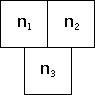
\includegraphics{img/pyramide3.pdf} 
\end{minipage}


\noindent Ce problème se pose par exemple lorsque l'on cherche à disposer les
boules de billards en respectant les contraintes données (dans ce cas,
$h=5$). Certaines instances du problème (certains $h$) n'admettent pas de
solution (cf. dernier exercice) tandis que d'autres admettent plusieurs
solutions (8 solutions pour $h=3$).

\begin{Exercice}\textbf{Représentation mémoire}
  \noindent La première idée pour représenter la pyramide est d'utiliser la
  moitié d'un tableau à deux dimensions de type \texttt{Array[Array[Int]]}, mais
  une seule moitié serait utilisée et l'autre serait réservée pour rien.
\end{Exercice}

\begin{figure}[h]
  \centering
  \includegraphics[scale=.9]{fig/ligne.fig}\vspace{-.5\baselineskip}
  \caption{Représentation mémoire contiguë.}
  \label{fig:mem}%\vspace{-1.5\baselineskip}
\end{figure}

\begin{wrapfigure}{r}{0.35\textwidth}
  \vspace{-1.2\baselineskip}
  \centerline{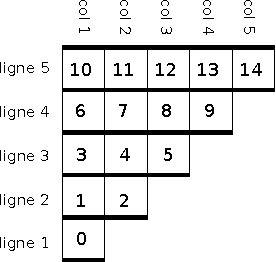
\includegraphics[scale=.9]{img/numerotation-ligne.pdf}}
  \vspace{-.5\baselineskip}
  \caption{Numérotation en ligne.}
  \label{fig:numligne}
  \vspace{-1.5\baselineskip}
  
\end{wrapfigure}

Pour économiser la mémoire, nous allons utiliser un tableau à une dimension en
rangeant les différentes «tranches de pyramides» les unes à coté des
autres. Selon la façon de couper ces tranches, il existe de nombreuses manières
de numéroter les cases. Nous allons pour instant prendre la plus simple, c'est à
dire numéroter les cases par lignes comme sur la figure ci-contre.

Il nous faut définir une fonction \texttt{indiceLigne(ligne,colonne)} calculant
l'indice de la case placée sur la \texttt{ligne} et sur la \texttt{colonne}
indiquée en suivant cette numérotation. Notez que:\\
\texttt{indiceLigne(1,1)=0} ; \texttt{indiceLigne(2,2)=2};\\
\texttt{indiceLigne(3,2)=4} ; \texttt{indiceLigne(4,2)=7}. 

\begin{Question}
  Écrivez cette fonction \texttt{indiceLigne(ligne,colonne)}, et explicitez ses préconditions.
  \noindent\textsc{Indication:} calculez le nombre de case dans la pyramide de
  hauteur \texttt{ligne}.
\end{Question}
\begin{Reponse}
  Pas la peine de les laisser bloquer trop longtemps sur ce problème, il n'en
  vaut pas la peine.
% On peut
%   leur donner assez rapidement, et les laisser chercher la question suivante,
%   plutôt.

\begin{Verbatim}
// précondition: 1 <= col <= lig <= hauteur 
def indiceLigne(lig:Int, col:Int): Int  =  lig * (lig - 1 ) / 2 + col - 1
\end{Verbatim}
(oui, scala permet de définir une fonction sur une ligne sans accolade de la sorte)
\end{Reponse}


% \begin{Question}
%   Écrivez \texttt{indiceColonne(ligne,col)} utilisant la numérotation par
%   colonnes de la figure~\ref{fig:numcol}.

%   \noindent\texttt{indiceColonne(1,1)=0} ; \hfill\texttt{indiceColonne(2,2)=2} ;
%   \hfill\texttt{indiceColonne(2,3)=4} ; \hfill\texttt{indiceColonne(2,4)=7}.
% \end{Question}
% \begin{Reponse}
% \begin{Verbatim}
% // précondition: lig >= 1 && lig <= hauteur() && diag >= lig && diag <= hauteur();
% def indiceColonne(lig:Int, diag:Int):Int = diag * (diag - 1 ) / 2 + lig - 1
% \end{Verbatim}
% \end{Reponse}

\begin{Exercice}\textbf{Algorithme «générer puis tester» (première approche)}

  \noindent La première idée est de générer toutes les pyramides existantes,
  puis de vérifier à postériori si elles vérifient les contraintes ou non. Il
  faut donc générer toutes les permutations de la liste des $n$ premiers
  entiers puis chercher celles vérifiant la seconde contrainte (puisque la
  première est vérifiée par construction).
\end{Exercice}

\begin{Question}
  Donnez un algorithme permettant de calculer les permutations des $n$ premiers
  entiers.
\end{Question}
\begin{Reponse}
  Générer les permutations est un code classique qu'il faut avoir vu une
  fois. C'est une bonne version simplifiée de ce qui vient après.  Quelques
  pistes pour les aider à trouver ce code:
  \begin{itemize}
  \item Énumérer à la main les permutations pour n=3 (321 312 231 213 132 123)
  \item Faire l'arbre d'appels comme on avait fait pour le knapsack, sauf qu'il
    n'y a pas un nombre constant d'éléments à chaque point
  \item Appliquer la recette de récursion classique:
    \begin{itemize}
    \item Paramètre de récursion: position en cours de remplissage (on a une
      permutation à sauvegarder)
    \item Cas trivial: quand la position est au delà du tableau
    \item Aide apportée par le bon génie: remplir correctement les positions suivantes
    \item Traitement à l'étage courant de récursion: Pour toutes les valeurs
      possibles, si une valeur n'est pas encore utilisée, la mettre et remplir
      le reste.
    \end{itemize}
  \item (vos idées sont bienvenues pour augmenter la liste)
  \end{itemize}
 
  \newcommand*\FancyVerbStopString{// Fin génération, début du test}
  \VerbatimInput{scala/permutations.scala}
\end{Reponse}

\begin{Question}
  Écrivez la fonction \texttt{correcte()} qui teste si une permutation donnée
  forme une pyramide valide. Il suffit de vérifier que chaque élément est la
  différence de ceux placés au dessus, puisque toutes les valeurs sont présentes
  par construction. La fonction \texttt{indiceLigne()} est utile ici.
\end{Question}
\begin{Reponse}
  On peut faire cette fonction en récursif (sur la ligne), mais c'est compliqué
  pour pas grand chose.

  \newcommand*\FancyVerbStopString{blablablabla}
  \newcommand*\FancyVerbStartString{// Fin génération, début du test}
  \VerbatimInput{scala/permutations.scala}
\end{Reponse}
\begin{Question}
  Sur machine, écrivez le code manquant pour trouver toutes les pyramides
  convenables de hauteur 3.
\end{Question}
\begin{Reponse}
  352164 341265 325461 314562 253614 235416 143625 134526

  Notez qu'il n'y en a que 4 d'originales, les autres sont symétriquement
  égales (dessinez-les). 
\end{Reponse}

\begin{Question}
  Dénombrez le nombre d'opérations que cet algorithme réalise.
\end{Question}
\begin{Reponse}
  \begin{itemize}
  \item Il y a $n!$ listes à construire
  \item Pour chacune, le processus de test est de complexité $O(n)$ car il y a
    $n$ cases à tester donc, le gros if au milieu sera appellé $n$ fois sur
    l'ensemble des appels.
  \end{itemize}
  La complexité est donc en $O(n\times n!)$, ce qui est \textbf{énorme}. Que
  ceux qui n'en sont pas convaincus tentent de calculer la hauteur 5 de cette
  façon. Moi j'ai craqué avant la fin de la génération de la hauteur 4.
\end{Reponse}

\begin{Exercice}\textbf{Algorithme de construction pas à pas (deuxième approche)}

  \noindent La solution de l'exercice précédent est inefficace car elle
  construit toutes les solutions possibles, même celles ne respectant pas toutes
  les contraintes du problème. Une amélioration possible consiste donc à
  vérifier à chaque étape de la construction que ces contraintes sont respectée,
  et à s'interrompre dès qu'un choix mène à une situation interdite.
  On appelle ce genre d'algorithmes des algorithmes récursifs avec retour
  arrière (\textit{backtracking algorithms} en anglais).

  \begin{Question}
    Modifiez la fonction correcte précédemment écrite\footnote{Lors du TP sur
      machine, vous devriez faire une copie de votre travail précédent afin de
      pouvoir comparer les versions.} afin qu'elle ne vérifie
    que le début du tableau, sans considérer les éléments placés après le
    paramètre \texttt{rang} qui ne sont pas initialisés.
  \end{Question}

  \begin{Reponse}
    \newcommand*\FancyVerbStartString{// BEGIN CORRECTE}
    \newcommand*\FancyVerbStopString{// END CORRECTE}
    \VerbatimInput{scala/lignes.scala}    
  \end{Reponse}

  \Question %
  Modifiez l'algorithme de génération des permutations écrit plus tôt afin de
  couper dès que la solution partiellement construite ne respecte pas la seconde
  contrainte du problème $n_1=\left|n_2-n_3\right|$

  \begin{Reponse}
    \newcommand*\FancyVerbStartString{// BEGIN GENERE}
    \newcommand*\FancyVerbStopString{// END GENERE}
    \VerbatimInput{scala/lignes.scala}    
  \end{Reponse}

  \Question %
  Sur machine, comparez le temps d'exécution de cette version avec celle de la
  version précédente pour la hauteur 3.  Si on mesure (avec la fonction
  System.nanotime) le temps $t_1$ avant l'opération et le temps $t_2$ après
  coup, la durée de l'opération en secondes est $\frac{t_2-t_1}{10^9}$.
\end{Exercice}

\ifcorrection{\newpage}{}
\begin{Exercice}\textbf{Génération par tranches (amélioration de l'approche)}
\end{Exercice}

\begin{wrapfigure}{r}{0.35\textwidth}
  \vspace{-.6\baselineskip}
  \centerline{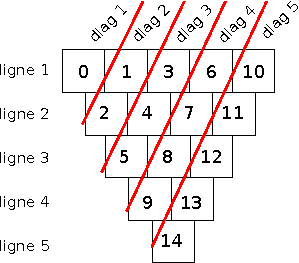
\includegraphics[scale=.9]{img/numerotation-diagonales.pdf}}
  \vspace{-.5\baselineskip}
  \caption{Numérotation diagonale.}
  \label{fig:numdiag}
   \vspace{-1.5\baselineskip}
\end{wrapfigure}

Couper les branches menant à des solutions invalides de la sorte s'avère
incroyablement plus rapide que la précédente. Cela permet de trouver des
pyramides de hauteur 5 en quelques secondes. Mais pour aller plus loin, il faut
raffiner cette approche.

Pour cela, l'objectif est de générer les contraintes le plus tôt possible, pour
s'éviter de d'agrandir des solutions partielles vouées à l'échec. Par exemple,
s'il s'avère impossible de placer une valeur dans la case 11 qui respecte les
contraintes, des cases comme 8, 9, 4, 5 ou 2 auront été remplies pour
rien. L'objectif est donc de changer l'ordre de remplissage pour détecter les
blocages le plus tôt possible et trouver les solutions plus vite.

L'approche «en colonnes» est préférable car la seconde contrainte lie un nombre
aux deux placés au dessus de lui. Il est donc naturel de chercher à traiter le
nombre du dessous juste après un nombre donné. Cela permet de s'assurer que
toute solution correcte aux étapes précédentes de la récursion ne gênera pas le
respect de la seconde contrainte. Au contraire, il est possible que l'approche
«en ligne» mène à une situation de blocage due à la seconde contrainte à l'étage
$n$ nécessitant de modifier les étages inférieurs.

\begin{Reponse}
  Avant d'aller plus loin, il faut motiver le travail prévu. Il faut faire
  sentir cette histoire de contrainte au plus tôt pour économiser des
  générations inutiles. Pour cela, les deux schémas suivants sont utiles:
  
  \begin{minipage}{.4\linewidth}
    \centering
    \includegraphics[scale=.8]{fig/pyramide-encours-ligne.fig}\vspace{-.5\baselineskip}
    
    Remplissage partiel par lignes.
  \end{minipage}\hfill
  \begin{minipage}{.4\linewidth} 
    \centering
    \includegraphics[scale=.8]{fig/pyramide-encours-col.fig}\vspace{-.5\baselineskip}
    
    Remplissage partiel par colonnes.
  \end{minipage}
\end{Reponse}

\Question %
Plutôt que de réaliser un parcours compliqué, nous allons renuméroter les cases
de la pyramide pour que l'ordre naturel expose les contraintes au plus
tôt. Écrivez une méthode \texttt{indiceDiag()} semblable à
\texttt{indiceLigne()} définie précédemment, mais numérotant les cases comme sur
la figure~\ref{fig:numdiag}.
 
\noindent\texttt{indiceDiag(1,1)=0} ; \hfill\texttt{indiceDiag(2,2)=2} ;
\hfill\texttt{indiceDiag(2,3)=4} ; \hfill\texttt{indiceDiag(2,4)=7}.
\begin{Reponse}
  Avec le code de indiceLigne , ils devraient parvenir à trouver celle-ci. Mais
  ce n'est pas la question la plus importante: si le temps manque il est
  préférable de leur donner pour réfléchir plutôt au reste.
  \begin{Verbatim}
// précondition: 1 <= ligne <= diag <= hauteur 
def indiceDiag(ligne:Int, diag:Int):Int = diag * (diag - 1 ) / 2 + ligne - 1
  \end{Verbatim}
\end{Reponse}

\Question %
Écrivez une nouvelle méthode \textbf{correcte()} vérifiant que la pyramide
respecte la seconde contrainte du problème dans le nouveau repère de numérotation.

\begin{Reponse}
  En fait, il suffit de changer l'ordre de parcours et les indices dans le calcul de $n_{123}$
  
  \newcommand*\FancyVerbStartString{// BEGIN CORRECTE}
  \newcommand*\FancyVerbStopString{// END CORRECTE}
  \VerbatimInput{scala/diagonales.scala}    
\end{Reponse}

\begin{Question}
  Sur machine, comparez le temps d'exécution de cette nouvelle version par
  rapport à la précédente (il n'est pas nécessaire de modifier la fonction de
  génération des permutations pour cela).
\end{Question}

\begin{Reponse}
  Il faut discuter un peu de pourquoi générer() reste la même, mais j'espère
  qu'ils verront vite qu'une permutation est une permutation, peu importe où
  sont placées les billes correspondantes dans le triangle.
  
  Voici des benchmarks imprécis réalisés sur ma machine. Ils ne sont pas
  réalisés avec une rigueur suffisante pour une publication, mais ils sont bien
  suffisants pour dire que notre nouvelle approche est décevante : on voit pas
  trop la différence.

  \begin{tabular}{|c|c|c|}\hline
    hauteur       &5&6\\\hline
    par lignes    &1.5s&40s\\\hline
    par diagonales&1.3s&39.5s\\\hline
  \end{tabular}
\end{Reponse}

\begin{Exercice}\textbf{Génération par propagation (amélioration de l'amélioration)}
\end{Exercice}

\noindent Les résultats pratiques obtenus à l'exercice précédent sont décevants,
et il faut encore affiner notre approche. Pour cela, on remarque qu'il est
inutile de tester toutes les valeurs possibles pour $n_3$ puis ne garder que
celles qui respectent les contraintes, car une fois que $n_1$ et $n_2$ sont
connus, une seule valeur est possible pour $n_3$. L'idée est alors de placer
une valeur possible en haut de la diagonale, puis de la propager en vérifiant
qu'on respecte la première contrainte. La seconde sera respectée par construction.

\Question %
Réécrivez l'algorithme sous forme d'une récursion portant sur la diagonale à
remplir et non sur chaque case de la pyramide comme précédemment. À chaque étage
de la récursion, il faut tester toutes les valeurs possibles à placer sur la
première ligne, à tour de rôle. Il faut ensuite propager cette valeur en
remplissant successivement les cases avec les valeurs imposées par la seconde
contrainte. Si la valeur à placer est déjà utilisée ailleurs dans la pyramide,
il faut couper court à la génération et explorer une autre branche. Si on
parvient à remplir cette diagonale, il faut (tenter de) remplir la suite par un
appel récursif sur la diagonale suivante. Vous aurez probablement besoin
d'écrire les fonctions suivantes:
\begin{itemize}
\item \texttt{contient(pyr:Array[Int], valeur:Int, rang:Int)} qui retourne vrai
  si la \texttt{valeur} est présente dans le début de la \texttt{pyr}amide
  (en ne considérant que les cases jusqu'à la position \texttt{rang}).
\item \texttt{propage(pyr:Array[Int], value:Int, diagonale:Int):Boolean} qui
  tente de propager cette \texttt{valeur} sur cette \texttt{diagonale} par une
  série de soustractions.
\item \texttt{genere(pyr:Array[Int], diagonale:Int)} qui tente de remplir
  récursivement la \texttt{pyr}amide sachant que toutes les diagonales
  inférieures à \texttt{diagonale} sont déjà remplies correctement. La condition
  d'arrêt de cette récursion est quand la pyramide est intégralement remplie, ou
  quand aucune valeur possible ne peut être propagée correctement.
\end{itemize}

\Question %
Sur machine, vérifiez que cette version retrouve toutes les solutions trouvées
par les algorithmes précédents. Chronométrez cette version de votre code pour
les hauteurs 5, 6 et 7. Ce problème n'admettant pas de solution pour $h=6$ ni
pour $h=7$, il est normal que votre code n'en trouve pas.

\begin{Exercice}\textbf{Pour aller plus loin}

\noindent\begin{minipage}{.7\linewidth}
    
  La figure ci-contre donne les temps de calcul (en secondes sur un centrino
  1.5Ghz) et les taux de remplissage obtenus pour des pyramides de différentes
  tailles. La dernière ligne indique donc que la recherche des pyramides de
  taille 12 a duré plus de 28h, et que la meilleure solution ne remplit que
  73\% du tableau.

  ~~~ Il semble donc que ce problème n'admette pas de solution pour $n>5$. On
  peut donc le généraliser de la façon suivante : on s'autorise à laisser de
  coté des nombres lors du remplissage de la pyramide. Il s'agit alors de
  minimiser le numéro $M$ de la plus grande valeur utilisée dans une pyramide à
  $n$ étages n'utilisant que des nombres entiers strictement positifs distincts
  tels que chaque valeur (sauf celles de la dernière ligne) soit la différence
  des deux valeurs situées immédiatement au-dessous.

  ~~~ Pour $n=5$, on a alors $M=\frac{n(n+1)}{2}=15$

  ~~~ Si vous trouvez une solution pour $n>5$, merci de la communiquer à
  l'équipe enseignante (qui n'en connait pas).

    
  \end{minipage}~~~\begin{minipage}{.3\linewidth}
%\begin{figure}[h]
%\centering
\begin{tabular}{|c|c|c|}
\hline
Rang & Remplissage & Temps\\
\hline
 2 &  3/3  & 0,002\\
 3 &  6/6  & 0,002\\
 4 & 10/10 & 0,003\\
 5 & 15/15 & 0,006\\
 6 & 20/21 & 0,12 \\
 7 & 25/28 & 0,9  \\
 8 & 31/36 & 6    \\
 9 & 37/45 & 70   \\
10 & 43/55 & 948  \\
11 & 49/66 & 11551\\
12 & 57/78 & 103671\\
\hline
\end{tabular}
%\caption{Relevé pour les rangs 1 à 12.}
%\label{tab:releve}
%\end{figure}

  \end{minipage}
  

\end{Exercice}

\begin{Reponse}
  Ca, c'est juste pour occuper ceux qui savent déjà programmer. Dites leur de
  m'envoyer leurs solutions par email privé...
\end{Reponse}
\end{document}
%%% Local Variables:
%%% coding: utf-8
